% Workshop draft. Generic layout approximating a NeurIPS/ICML workshop page (5.5in text width, 10pt).
% Before submission: move the body into the workshop's official style file and check its page limit.
\documentclass[10pt]{article}
\usepackage[textwidth=5.5in,textheight=9in,centering]{geometry}
\usepackage[T1]{fontenc}
\usepackage{lmodern}
\usepackage{microtype}
\usepackage{amsmath,amssymb}
\usepackage{booktabs}
\usepackage{xcolor}
\usepackage[hidelinks]{hyperref}
\usepackage[numbers,sort&compress]{natbib}
\usepackage{caption}
\usepackage{pgfplots}
\pgfplotsset{compat=1.18}
\captionsetup{font=small,labelfont=bf}

\definecolor{orig}{HTML}{9AA6A4}
\definecolor{rep}{HTML}{0F6B63}
\definecolor{posc}{HTML}{A8402C}
\definecolor{negc}{HTML}{2C5F9E}

\newcommand{\uhat}{\hat{u}}
\newcommand{\asym}{\mathrm{asym}}

\title{Normal Scans, Unmoved Beliefs:\\Diagnosing and Repairing Under-Used Negative Evidence in a Clinical LLM}
\author{Anonymous Authors}
\date{}

\begin{document}
\maketitle

\begin{abstract}
How much a test result should change a diagnosis is fixed by the test's accuracy: its likelihood ratio gives a prior-independent target shift in log-odds. We use this yardstick to audit an open-weight LLM (Qwen3.5-9B) on real emergency-department histories from MIMIC-IV. Across five imaging tests and 19 report wordings, positive reports move the model's belief as much as the literature warrants or more, while negative reports are under-weighted relative to positives in every wording. A CT report stating only that the sigmoid colon is normal moves belief by 0.25 log-odds against a target of 2.80, and raises belief in diverticulitis in 48 of 103 cases. Blood-test negatives show no such deficit. Inside the model, negative results are read and written into the residual stream about as strongly as positive ones. The difference lies in conversion: later layers turn a positive's off-axis content into movement along the Yes--No readout direction, but do much less with an imaging negative's. A selective rank-1 weight edit (0.02\% of parameters), found by an LLM agent under a fixed evaluation harness, supplies the missing conversion. On held-out patients, wordings and tests it cuts the positive/negative imbalance from 0.91 to 0.30 (random edits of the same size: 0.89--0.92). Wrong-direction negatives fall from 79 to 2, and blood tests, pending-result beliefs and general questions are left essentially unchanged.
\end{abstract}

\section{Introduction}

Ruling a diagnosis out is as much part of diagnosis as ruling it in. A clinical assistant that discounts a normal scan keeps suspected diagnoses alive and invites unnecessary follow-up. Accuracy benchmarks rarely expose this, because a model can name the right diagnosis most of the time and still update on evidence in the wrong proportions.

Evidence use has a normative yardstick. A result multiplies the odds of disease by its likelihood ratio (LR), so on the log-odds scale a positive result should raise belief by $\ln \mathrm{LR}^{+}$ and a negative one should lower it by $-\ln \mathrm{LR}^{-}$, whatever the prior. We compare an LLM's belief shifts against these targets and ask three questions. Is there a systematic gap? Where in the network does it arise? Can a small, selective weight edit close it without side effects?

\paragraph{Contributions.}
(1) A likelihood-ratio audit showing a consistent \emph{positive-evidence bias} for imaging results in Qwen3.5-9B: negatives are under-weighted relative to positives in 19/19 imaging wordings, and blood tests do not share the deficit (\S\ref{sec:bias}).
(2) A selective rank-1 repair, found by an LLM agent through a rule-enforcing harness and scored by us on a held-out set it never saw, that removes two thirds of the imbalance and generalises to unseen imaging tests (\S\ref{sec:repair}).
(3) A mechanistic account read backwards from the repair. Negative results are encoded but not converted to the readout axis; lab and imaging negatives are nearly identical in their shared content, which is why the repair must be selective; and the bias grows with the number of inference steps between a reported finding and the asked disease (\S\ref{sec:mech}).

\section{Setup}\label{sec:setup}

\paragraph{Cases and prompts.} We use 188 emergency-department histories from the MIMIC-IV clinical decision-making cohort \citep{johnson2023mimiciv,hager2024evaluation}, covering appendicitis, cholecystitis, diverticulitis and pancreatitis. We remove every sentence mentioning imaging, laboratory tests, the diagnosis or any candidate disease. Each prompt holds a history, one ``New test result'' line, and the question ``Does this patient have \emph{[disease]}? Answer Yes or No only.'' For each history and test we build three prompts that differ only in the result line: \textbf{B} (``result pending''), \textbf{P} (a positive report) and \textbf{N} (a negative report). Every history is combined with every test, whatever the patient's true diagnosis.

\paragraph{Belief and moves.} We read belief at the answer position as $m = \mathrm{logit}(\text{Yes}) - \mathrm{logit}(\text{No})$, the log-odds of Yes over No. The model's moves are $\mathrm{up} = m(P) - m(B)$ and $\mathrm{down} = m(B) - m(N)$, so the history cancels and only the result line is judged. We keep \emph{mid-prior} cases, where $P(\text{Yes} \mid B) \in [0.02, 0.95]$; near the extremes, moves saturate for reasons unrelated to evidence use.

\paragraph{Tests and yardstick.} Seven tests, each paired with its target disease: CT for diverticulitis \citep{lameris2008diverticulitis}, appendicitis and kidney stones \citep{lit_ct_stone}; ultrasound (US) for cholecystitis \citep{lit_us_gallbladder} and appendicitis \citep{lit_us_appendix}; serum lipase and amylase for pancreatitis \citep{lit_amylase}. Ideal moves are $\ln(\text{sens}/(1-\text{spec}))$ up and $\ln(\text{spec}/(1-\text{sens}))$ down. For CT in diverticulitis (sensitivity 0.94, specificity 0.99) these are 4.54 and 2.80. Each test has 2--6 positive/negative wordings modelled on real reports, ranging from naming the disease (``No evidence of diverticulitis'') to describing only the organ (``The sigmoid colon and rectum are normal in appearance'').

\paragraph{Metric.} Overall move size is miscalibrated in a test-dependent way. Positive moves are at or above target for every test, and negative moves are too small for CT but too large for blood tests. We factor out a common scale and compare only the two moves relative to each other:
\begin{equation}
\asym = \ln\frac{\mathrm{up}}{\mathrm{down}} - \ln\frac{\mathrm{up}^{*}}{\mathrm{down}^{*}},
\end{equation}
where $^{*}$ marks the literature moves. $\asym > 0$ means negatives are under-weighted relative to positives. A repair is scored by the mean of $|\asym|$ over (test, wording) cells. Dropping the sign stops over- and under-weighting from cancelling and penalises overshoot. A score of 0.91 means the up/down ratio is off by a factor of $e^{0.91}\approx 2.5$.

\section{The bias}\label{sec:bias}

\begin{table}[t]
\centering\small
\caption{Positive-evidence bias on 94 held-out histories (mid-prior cases per test: 50--92). Moves are the model's mean divided by the literature move (1 = exact). ``Wrong way'': case--wording pairs where a negative report \emph{raised} belief.}
\label{tab:bias}
\setlength{\tabcolsep}{4pt}\footnotesize
\begin{tabular}{lcccccr}
\toprule
test & sens/spec & up $\div$ ideal & down $\div$ ideal & mean $\asym$ & wordings $\asym{>}0$ & wrong way \\
\midrule
CT diverticulitis & .94/.99 & 1.01 & \textbf{0.33} & $+1.41$ & 6/6 & 62/300 \\
CT kidney stone   & .96/.94 & 1.81 & \textbf{0.58} & $+1.14$ & 2/2 & 0/178 \\
CT appendicitis   & .95/.94 & 1.66 & \textbf{0.68} & $+0.91$ & 6/6 & 9/420 \\
US cholecystitis  & .71/.85 & 3.26 & 1.49 & $+0.81$ & 3/3 & 6/222 \\
US appendicitis   & .82/.86 & 2.18 & 0.97 & $+0.79$ & 2/2 & 2/184 \\
\midrule
Serum lipase      & .77/.92 & 1.22 & 1.81 & $-0.40$ & 0/3 & 0/249 \\
Serum amylase     & .72/.93 & 1.27 & 1.58 & $-0.22$ & 0/2 & 0/144 \\
\bottomrule
\end{tabular}
\end{table}

Table~\ref{tab:bias} summarises the audit. Every imaging wording has $\asym > 0$. For CT the deficit is absolute: negatives move belief only 33--68\% as far as they should while positives meet or exceed their target. For ultrasound, negatives are roughly on target but positives overshoot 2--3$\times$, so negatives are still under-weighted relative to positives. Both blood tests lean slightly the other way.

Wording matters most. On all 188 histories, for CT in diverticulitis (n=103 mid-prior), the up/down ratio is 2.36 (95\% bootstrap CI 2.12--2.62) for ``No evidence of diverticulitis'', against a literature range of 1.13--1.62. It rises to 19.5 (10.9--79.6) for ``The sigmoid colon and rectum are normal in appearance''. That sentence moves belief by 0.25 log-odds against a target of 2.80, and raises belief in 48 of 103 cases. A patient at 50\% should fall to about 6\%; the model ends near 44\%.

\section{Repair}\label{sec:repair}

\paragraph{Protocol.} The repair was searched for by an LLM coding agent (Claude Code) acting as researcher. It could touch the model only through a server that holds the weights, enforces the rules and keeps a budget of 80 scoring calls and 5{,}000 probe prompts. The rules forbade edits to embeddings, unembedding and final norm, and capped any edit at 5M weights. The agent saw only a practice split: 94 histories, CT diverticulitis and appendicitis, and lipase as a ``do not break'' control. Success criteria were fixed before the search. The score had to fall clearly; lipase $|\asym|$ could worsen by at most 0.1; and wrong-direction negatives had to fall. Guards required that mean drift of the pending-result belief $|m'(B)-m(B)|$ stay below 0.15, that 40/40 general-knowledge Yes/No questions remain correct, and that language-modelling loss on the histories change by less than 0.01. After delivery we scored every edit on a held-out set: 94 new histories, new wordings (including negatives with neither a negation word nor the disease name) and four new tests (both ultrasounds, kidney-stone CT and amylase).

\paragraph{The edit.} The best edit that passes every guard (C3) has two rank-1 parts, about 2.1M weights (0.02\% of the model). In the layer-28 Gated DeltaNet mixer \citep{yang2025gateddelta}, a rank-1 change to the output projection reads a direction fitted by ridge regression and writes the mixer's own mean output for \emph{blood-test negatives}. One rarely used neuron in MLP 31 is repurposed as a linear read-out whose output weight is $-\uhat$, the model's Yes--No readout direction (\S\ref{sec:mech}), at 0.75 strength. Both read vectors share one target. They fire on under-used imaging negatives ($N{-}B \to +k$) and stay silent on lipase negatives, positives, pending prompts, general questions and all non-answer tokens ($\to 0$). Nothing in the model is removed.

\begin{figure}[t]
\centering
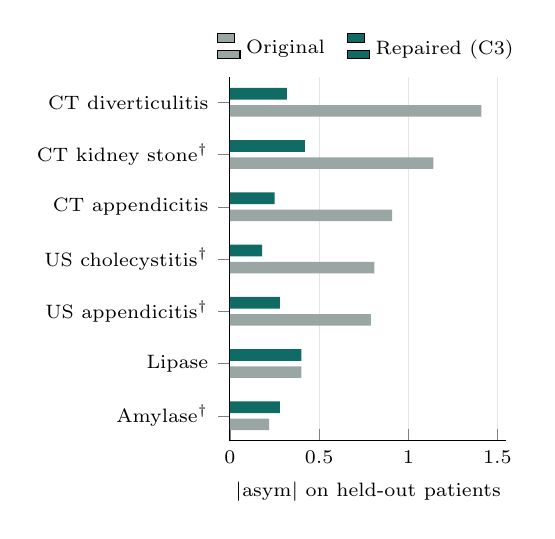
\begin{tikzpicture}
\begin{axis}[
  xbar, width=0.42\linewidth, height=6.2cm,
  bar width=4.2pt, xmin=0, xmax=1.55,
  symbolic y coords={Amylase$^\dagger$,Lipase,US appendicitis$^\dagger$,US cholecystitis$^\dagger$,CT appendicitis,CT kidney stone$^\dagger$,CT diverticulitis},
  ytick=data, y tick label style={font=\scriptsize}, x tick label style={font=\scriptsize},
  xlabel={$|\asym|$ on held-out patients}, xlabel style={font=\scriptsize},
  legend style={font=\scriptsize, at={(0.5,1.02)}, anchor=south, draw=none, legend columns=2, /tikz/every even column/.append style={column sep=6pt}},
  enlarge y limits=0.08, axis x line*=bottom, axis y line*=left,
  xmajorgrids, grid style={gray!20},
]
\addplot[fill=orig, draw=none] coordinates {(0.22,Amylase$^\dagger$) (0.40,Lipase) (0.79,US appendicitis$^\dagger$) (0.81,US cholecystitis$^\dagger$) (0.91,CT appendicitis) (1.14,CT kidney stone$^\dagger$) (1.41,CT diverticulitis)};
\addplot[fill=rep, draw=none] coordinates {(0.28,Amylase$^\dagger$) (0.40,Lipase) (0.28,US appendicitis$^\dagger$) (0.18,US cholecystitis$^\dagger$) (0.25,CT appendicitis) (0.42,CT kidney stone$^\dagger$) (0.32,CT diverticulitis)};
\legend{Original, Repaired (C3)}
\end{axis}
\end{tikzpicture}\hfill
\begin{minipage}[b]{0.3\linewidth}\footnotesize
\begin{tabular}{@{}lc@{}}
\toprule
 & score \\
\midrule
original & 0.91 \\
random edits & 0.89--0.92 \\
\textbf{C3} & \textbf{0.30} \\
\midrule
\multicolumn{2}{@{}l}{\emph{by subset (orig.\,$\to$\,C3)}}\\
seen tests & 0.87\,$\to$\,0.26 \\
new wordings & 1.28\,$\to$\,0.41 \\
new tests & 0.75\,$\to$\,0.28 \\
\midrule
wrong-way neg. & 79\,$\to$\,2 \\
pending drift & 0.13 \\
\bottomrule
\end{tabular}\vspace{2pt}
\end{minipage}
\caption{Held-out results. Left: per-test imbalance before and after the repair; $^\dagger$ tests never seen during the search. Right: overall score (mean $|\asym|$ over cells), its split by what is new, wrong-direction negatives (random edits: 77--78), and pending-result drift (guard 0.15).}
\label{fig:repair}
\end{figure}

\paragraph{Results.} Figure~\ref{fig:repair} shows the held-out results. The score falls from 0.91 to 0.30, while random edits of the same size at the same places leave it at 0.89--0.92. The more biased a test was, the more is removed. CT diverticulitis falls by 1.09 and US appendicitis by 0.51, and all five imaging tests end in a narrow band (0.18--0.42). The gain transfers to three imaging tests never seen in the search, which differ in modality, organ and disease. Lipase is unchanged and amylase moves slightly (0.22 $\to$ 0.28). Negatives that pushed belief the wrong way fall from 79 to 2. Pending-result drift is 0.13, general questions stay at 40/40, and history loss changes by at most 0.0015. For a negative wording with no negation word and no disease name (``The sigmoid colon has a normal wall thickness and the surrounding fat is clear''), wrong-direction cases fall from 24 to 1.

\paragraph{Why selectivity matters.} An earlier, non-selective edit in one late attention head read ``negative result'' and wrote ``No''. It fixed imaging but pushed lipase $|\asym|$ from 0.36 to 0.69 and drifted pending beliefs by 0.161. That practice set held only CT tests, so the overshoot was invisible to the agent. Adding lipase to practice was enough for the agent to find a selective read on its own.

\section{What the repair reveals}\label{sec:mech}

A fix that works is also evidence about the failure. We use the readout direction $\uhat = (1+g)\odot(W_U[\text{Yes}] - W_U[\text{No}])$, where $g$ is the final RMSNorm weight, so that $m \approx (h/\mathrm{rms}(h))\cdot\uhat$. This is exact at the final layer and serves as a logit-lens gauge \citep{nostalgebraist2020logitlens} at layers 25--29. A result's \emph{displacement} at layer $\ell$ is the mean over patients of $h_\ell(X) - h_\ell(B)$ at the answer position, with $X \in \{P, N\}$. We call its component along $\uhat$ \emph{on-axis} and the rest \emph{off-axis}. Interventions add or remove directions in the residual stream \citep{turner2023actadd,zhang2024patching}, always with matched random controls.

\paragraph{Negatives are read, not ignored.} Positive and negative displacements have similar norms (ratio 1.1--1.26). Both move from the report tokens to the answer position at the same depth: on the report up to layer 12, at the answer by layer 20. That a single linear read separates under-used imaging negatives from well-used lab negatives at layers 26, 27, 28 and 31 says the same thing. The information is present; it is not carried to ``No''.

\paragraph{A general ``evidence-against'' direction.} Let $d_V$ be the layer-29 negative displacement with its component along the positive displacement removed. Removing $d_V$ abolishes the negative move (1.49 $\to$ $-0.15$) and leaves positives intact. Adding it to pending prompts lowers belief by 1.66, and adding it to general questions whose answer is Yes pushes them toward No. The same sentence writes nearly the same $d_V$ across patients (correlation 0.87). Observationally, $d_V$ encodes evidence against the asked disease rather than negation. A positive finding for a \emph{different} disease projects onto it as strongly as a true negative (cosine 0.93 with the negative's off-axis part), while a negated history sentence (``denies fever'') does not ($-0.04$). $d_V$ is written gradually by many components in layers 19--29, none contributing more than 11\%.

\begin{figure}[t]
\centering
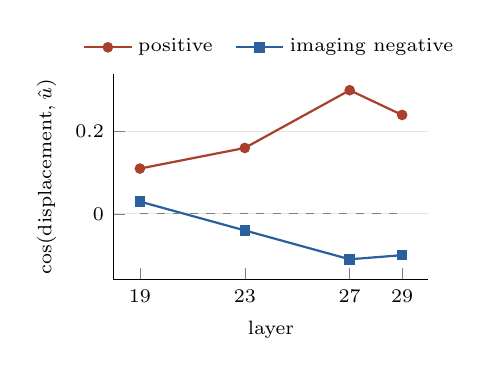
\begin{tikzpicture}
\begin{axis}[
  width=0.46\linewidth, height=4.2cm,
  xlabel={layer}, ylabel={$\cos(\text{displacement}, \uhat)$},
  xtick={19,23,27,29}, ymin=-0.16, ymax=0.34,
  label style={font=\scriptsize}, tick label style={font=\scriptsize},
  legend style={font=\scriptsize, at={(0.5,1.03)}, anchor=south, draw=none, legend columns=2, /tikz/every even column/.append style={column sep=6pt}},
  axis x line*=bottom, axis y line*=left, ymajorgrids, grid style={gray!20},
]
\addplot[posc, thick, mark=*, mark size=1.5pt] coordinates {(19,0.11) (23,0.16) (27,0.30) (29,0.24)};
\addplot[negc, thick, mark=square*, mark size=1.5pt] coordinates {(19,0.03) (23,-0.04) (27,-0.11) (29,-0.10)};
\addplot[gray, dashed, domain=19:29] {0};
\legend{positive, imaging negative}
\end{axis}
\end{tikzpicture}\hfill
\begin{minipage}[b]{0.5\linewidth}\small
\begin{tabular}{@{}lcc@{}}
\toprule
off-axis part removed at & L29 & L25 \\
\midrule
loss of positive move (4.68) & 19\% & 29\% \\
loss of negative move (1.49) & 10\% & 19\% \\
\bottomrule
\end{tabular}\\[6pt]
Adding the positive's off-axis part alone to $B$ at L29: $+0.72$. Adding the negative's off-axis part (99.5\% of its displacement): no more than a random direction.
\end{minipage}
\caption{Recycling of off-axis content. Left: the on-axis share of the displacement grows with depth for positives, much less for imaging negatives (a random direction has $|\cos| \approx 0.016$ in 4096 dimensions). Right: removing the off-axis part earlier costs more, the signature of step-by-step conversion, and the cost is larger for positives.}
\label{fig:recycle}
\end{figure}

\paragraph{Positives are recycled into Yes; imaging negatives are not.} Almost every displacement is mostly off-axis, positives included. What differs is whether later layers convert off-axis content into movement along $\uhat$ (Fig.~\ref{fig:recycle}). The positive's on-axis share grows from 0.11 at layer 19 to 0.30 at layer 27. Its off-axis part alone raises belief by 0.72, and removing it costs more the earlier it is removed. The imaging negative's off-axis part behaves like a random direction. The conversion is concentrated: heads 27.11 and 27.13 and the layer-28 mixer write Yes for positives (the mixer $+1.76$) and nearly nothing for imaging negatives. Lab negatives \emph{are} converted, via head 27.12, head 23.5 and MLPs 23--28. The repair copies this lab route: its layer-28 part makes the mixer answer an imaging negative as it already answers a lab negative.

\paragraph{The read must be selective.} Lab and imaging negatives write nearly the same content (cosine 0.85--0.89 between displacements) and differ mainly in their small on-axis part ($-0.12$ for lab, $-0.03$ to $-0.05$ for CT). Any read of the shared content cannot tell them apart, which explains why the non-selective edit overshot lipase.

\paragraph{There is nothing to remove, and placement matters.} Every working edit adds a pathway. None of three candidate obstacles held up. Final-layer ``damping'' neurons shrink all judgements proportionally. A neutral ``result arrived'' component does not push toward Yes. Removing an ``organ mentioned'' component makes the bias worse (1.12 $\to$ 1.52). Placement matters because of self-repair \citep{mcgrath2023hydra}. Layers 27--31 cancel 85--90\% of a ``No'' written into MLPs 26--27, and MLP 31 cancels about half of any late change. A write into the layer-28 mixer is instead amplified by the layer-28 MLP, and MLP 31, as the last writer, cannot be overruled. From practice to held-out, pending drift grew about $3\times$ for the MLP-31 read but only $1.2\times$ for the layer-28 read, which is why the best edit splits the work between them.

\paragraph{Inference distance limits the repair.} The hardest cells after repair ($\asym$ from $+0.3$ to $+0.9$) are organ-level negatives. ``Appendix normal'' rules out appendicitis in one step; ``sigmoid colon normal'' needs a second, because diverticulitis is inflammation of pouches (diverticula) in the colon wall. Changing only the negative sentence (24 histories) gives the following shares of the literature move. Sigmoid original: 1\%; without ``and rectum'': 9\%; naming the diverticula (``No diverticula or inflammation in the sigmoid colon''): 86\%. Appendix original: 74\%; one step further out (``The right lower abdomen is normal''): 50\%. The second pair has no lexical overlap with the disease name, so the effect is not just word matching. The failing sentences already produce short displacements at layer 19 (norm 7.8 vs.\ 11.6--13.7 for working negatives). The deficit thus starts upstream of every edit we tried, and the repair compensates for it downstream.

\section{Related work}

Language models handle negation poorly \citep{ettinger2020bert,kassner2020negated,truong2023naysayers}. Our object differs: a negative \emph{test result}, often with no negation word, judged against a quantitative target that makes both under- and over-use measurable. LLM clinical decision-making on MIMIC-IV has been evaluated mainly for diagnostic accuracy \citep{hager2024evaluation}; we measure belief updating. Methodologically we build on activation patching and circuit analysis \citep{wang2023ioi,zhang2024patching}, the logit lens \citep{nostalgebraist2020logitlens}, linear representations \citep{marks2023geometry}, self-repair \citep{mcgrath2023hydra} and rank-1 weight editing \citep{meng2022rome}. Here the edit targets an evidence-weighting failure rather than a stored fact.

\section{Limitations and next steps}

\textbf{One model.} All results are for Qwen3.5-9B \citep{qwen35}. Whether other models, including medically tuned ones such as MedGemma, share the bias is the most important open question. The behavioural audit (\S\ref{sec:bias}) needs only logits and transfers directly; the mechanism and repair would need to be re-derived. \textbf{One format and a narrow domain.} We use a binary question on acute abdominal conditions. In a four-way multiple-choice format, negatives were even more skewed but confounded by topic priming. \textbf{Yardstick.} Literature LRs are population averages that assume test accuracy is independent of history; our claim concerns a systematic, direction-consistent gap, not single cases. \textbf{Overall calibration} is out of scope: the ratio metric deliberately ignores it, and ultrasound positives remain 2--3$\times$ too strong. \textbf{Edit selection.} Lower-strength fallbacks were listed by the agent before held-out scoring, but we evaluated them only after the strongest edits exceeded the drift guard. All delivered edits and fallbacks are reported in Appendix~\ref{app:edits}. Held-out per-test scores are point estimates without confidence intervals. \textbf{The ``imaging vs.\ lab'' line may be approximate.} In a small check, urinalysis and white-cell-count negatives were also under-used, while an hCG negative was used fully.

\bibliographystyle{plainnat}
\bibliography{refs}

\appendix
\section{All delivered edits on the held-out set}\label{app:edits}

\begin{table}[h]
\centering\small
\caption{Search arms and held-out scores. Every score column is mean $|\asym|$ over cells; subsets hold different numbers of cells, so the overall score is not their plain mean. General accuracy stayed 40/40 and history loss changed by $\le 0.0015$ for every edit. Arms: A, anything in layers 30--31; B, attention/mixer in layers 23--29 (no MLPs); C, unrestricted.}
\setlength{\tabcolsep}{3.5pt}\footnotesize
\begin{tabular}{llcccccc}
\toprule
edit & where & score & seen & new wordings & new tests & wrong way & drift \\
\midrule
original & -- & 0.910 & 0.87 & 1.28 & 0.75 & 79 & 0 \\
random controls & same places/sizes & 0.89--0.92 & & & & 77--78 & -- \\
A $\times$1.5 & MLP31 neuron & 0.298 & 0.26 & 0.36 & 0.31 & 0 & \textcolor{posc}{0.168} \\
A $\times$1.0 & MLP31 neuron & 0.355 & 0.30 & 0.47 & 0.35 & 3 & 0.113 \\
B k10 & L28 mixer & 0.301 & 0.26 & 0.43 & 0.27 & 3 & 0.132 \\
B k8  & L28 mixer & 0.360 & 0.31 & 0.52 & 0.32 & 13 & 0.107 \\
C5 & MLP26/27 + MLP31 & 0.306 & 0.25 & 0.41 & 0.31 & 0 & \textcolor{posc}{0.235} \\
\textbf{C3} & L28 mixer + MLP31 & \textbf{0.296} & 0.26 & 0.41 & 0.28 & 2 & 0.126 \\
\bottomrule
\end{tabular}
\end{table}

\section{Read-vector fitting targets}
Both read vectors are fitted by ridge regression on the input of the edited component, at the answer position, with targets: imaging $N - B \to +k$; lipase $N - B \to 0$; any $P - B \to 0$; pending $B \to 0$; 40 general Yes/No questions $\to 0$; all non-answer tokens $\to 0$. The last group was necessary: without it the mixer edit fired mid-prompt.

\section{Data use}
MIMIC-IV was accessed under the PhysioNet credentialed data use agreement. The model ran on local hardware with open weights. % TODO(author): state precisely what the search agent could see (aggregate scores only, or prompt text?) and confirm compliance with PhysioNet's policy on LLM services.
No patient text appears in this paper.

\end{document}
